\chapter{JDBC~项目}

\section{整体概述}
JDBC项目是实践第一个项目,目的实现简易的外卖平台后台管理程序。通过java提供的jdbc数据库连接接口实现对数据库的操作。

\section{设计}
\subsection{功能描述}
整个项目有两个大的功能,商家管理和商家商品列表管理。管理员通过输入管理员用户名和密码可以进入后台查询、更新、删除商家信息;商家可以输入商家用户名和密码查询、更新密码页面、删除商家信息。

\subsection{数据设计}
实体类:

Admin(管理员):私有变量(管理员ID:adminId(Integer)、管理员用户名:adminName(String)、密码password(String))

Business(商家):私有变量(商家ID:businessId(Integer)、商家名称:businessName(String)、密码:password(String)、商家地址:businessAddress(String)、
商家描述信息:businessExplain(String)、起送费:starPrice(Double)、配送费:deliveryPrice(Double))

Food(商品):私有变量(商品ID:foodId(Integer)、商品名:foodName(String)、商品描述信息:foodExplain(String)、价格:(Double)、所属商家ID:businessId(Integer)

工具类:

DBUtil(数据库连接工具):私有静态变量:DataSource(连接池工具,用来实现数据库持久连接)


\subsection{数据库设计}
   \begin{table}[htbp]
    	\caption{admin表}\label{tab:table_6_10}
    	\vspace{0.5em}\wuhao
    	\begin{tabularx}{\hsize}{@{\extracolsep{\fill}}c c c}
    		\toprule[1.5pt]
    		字段名          &  数据类型  &   说明 \\ 
    		\midrule[1pt]
    		adminId & INT & 管理员ID \\
    		adminName & varchar & 管理员用户名 \\
    		password & varchar & 密码 \\
    		\bottomrule[1.5pt]
    	\end{tabularx}
    	\vspace{\baselineskip}
    \end{table}
    
    \begin{table}[htbp]
    	\caption{business表}\label{tab:table_6_10}
    	\vspace{0.5em}\wuhao
    	\begin{tabularx}{\hsize}{@{\extracolsep{\fill}}c c c}
    		\toprule[1.5pt]
    		字段名          &  数据类型  &   说明 \\ 
    		\midrule[1pt]
    		businessId & INT & 商家ID \\
    		businessName & varchar & 商家名 \\
    		password & varchar & 密码 \\
    		businessAddress & varchar & 商家地址 \\
    		businessExplain & varchar & 商家描述信息 \\
    		deliveryPrice & decimal & 配送费 \\
    		starPrice & decimal & 起送费 \\
    		\bottomrule[1.5pt]
    	\end{tabularx}
    	\vspace{\baselineskip}
    \end{table}
 
     \begin{table}[htbp]
    	\caption{business表}\label{tab:table_6_10}
    	\vspace{0.5em}\wuhao
    	\begin{tabularx}{\hsize}{@{\extracolsep{\fill}}c c c}
    		\toprule[1.5pt]
    		字段名          &  数据类型  &   说明 \\ 
    		\midrule[1pt]
    		foodId & INT & 商品ID \\
    		businessId & INT & 所属商家ID \\
    		foodName & varchar & 商品名 \\
    		foodExplain & varchar & 商品描述信息 \\
    		foodPrice & decimal & 商品价格 \\
    		\bottomrule[1.5pt]
    	\end{tabularx}
    	\vspace{\baselineskip}
    \end{table}
\subsection{程序结构}
应用一共分成三个层次:

view层:该层是为了给用户提供简易的与后台交互的界面。

po层:将数据库表格数据映射成JAVA程序能操作的对象实体。

Dao层:实现对数据库的操作

其中Dao层和View层分成抽象接口和继承接口的Impl对象来实现解耦操作。
\subsection{结构图}

\begin{figure}[htbp]
	\centering
	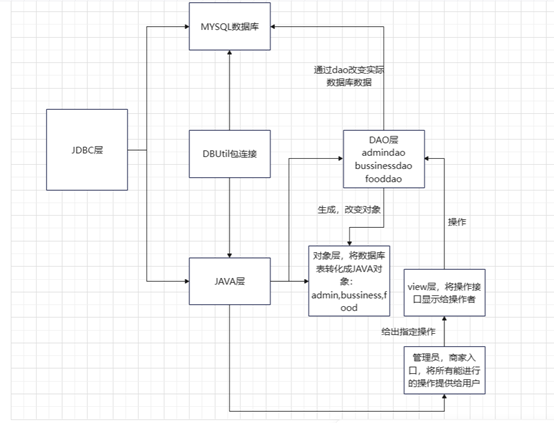
\includegraphics[width=0.8\textwidth]{jdbc}
	\caption{jdbc结构图}
	\vspace{\baselineskip}
\end{figure}
\subsection{操作数据库接口描述}
\subsubsection{Admin}
\textbf{获取管理员对象}

getAdminByNameByPass

参数:adminName(String),password(String)

返回值:Admin

功能:传入管理员用户名和密码查找并返回对应的管理员实体。

\subsubsection{Business}
\textbf{列出商家}

listBusiness

参数:businessName(String),businessAddress(String)

返回值:List<Business>

功能:通过传入商家名和地址列出相关商家

\textbf{存储商家}

saveBusiness

参数:businessName(String)

返回值:int

功能:通过输入商家名存储商家到数据库

\textbf{删除商家}

removeBusiness

参数:businessId(int)

返回值:int

功能:通过传入商家Id在数据库中删除对应商家

\textbf{获取商家}

getBusinessByIdByPass

参数:businessId(Integer),password(String)

返回值:Business

功能:通过商家ID和密码返回商家

\textbf{管理员获取商家}

getBusinessById

参数:businessId(Integer)

返回值:Business

功能:通过商家ID返回商家

\textbf{更新商家信息}

updateBusiness

参数:business(Business)

返回值:int

功能:传入商家实体,将表中ID相同的商家信息修改为实体对象对应的信息

\textbf{修改商家密码}

updateBusinessByPassword

参数:businessId(Integer),password(String)

返回值:int

功能:通过传入商家Id,将对应数据库中的商家密码修改成传入的密码

\subsubsection{Food}
\textbf{列出商家商品}

listFoodByBusinessId

参数:businessId(Integer)

返回值:List<Food>

功能:查询数据库,列出商家ID对应商家的商品列表

\textbf{存储商品}

saveFood

参数:food(Food)

返回值:int

功能:将商品存进商品数据库表

\textbf{获取商品}

getFoodById

参数:foodId(Integer)

返回值:Food

功能:通过商品ID查询数据库并返回对应商品

\textbf{更新商品信息}

updateFood

参数:food(Food)

返回值:int

功能:通过传入的商品实体对象,更新数据库中商品ID相同的商品信息

\textbf{删除商品}

removeFood

参数:foodId(Integer)

返回值:int

功能:删除数据库商品表中对应商品ID的商品信息

\subsection{软件对外界的接口}
\textbf{管理员入口}

ElmAdminEntry

功能:输入用户名和密码登录管理员,并能够选择对应数据库的操作。

\textbf{商家入口}

ElmBusinessEntry

功能:输入用户名和密码登录商家,并能够选择对应数据库的操作。

\section{部署}
通过打包成jar包,可以在windows控制台直接运行,具体情况如图
\begin{figure}[htbp]
	\centering
	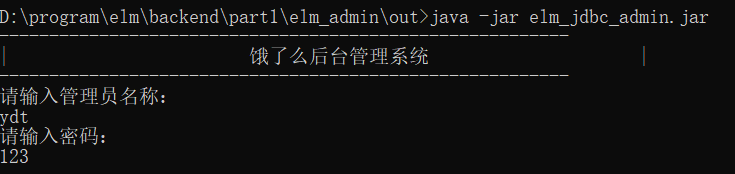
\includegraphics[width=0.8\textwidth]{jdbcres}
	\caption{运行情况}
	\vspace{\baselineskip}
\end{figure}